%%%%%%% TOOLS %%%%%%
\section{Libraries and technologies}
\label{libraries_and_technologies}

This section covers the different libraries and technologies used in the development of this thesis. First, the programming framework present in the project's progression is displayed, as well as the different third-party libraries and packages that has been employed in the software. Afterwards, the tools used for profiling and testing the code are analyzed and, finally, the hardware being used is presented and its main characteristics explained. 




	\subsection{ROS}
		\label{ros}

	ROS is the acronym of Robot Operating System\cite{ros}. It is an open source set of libraries and various tools that are aimed at robot applications. It is intended as well to improve the efficacy of collaborative robotics development, allowing easy interconnection of ROS packages. 


	\begin{figure}[h]
		\begin{center}
	    
\includegraphics[scale=0.3]{img/ros/groovy.eps}
		\caption[ROS Groovy Logo]{ROS Groovy Logo}
		\end{center}
	\end{figure}

	The tools, libraries and third-party packages available in the different ROS distributions are very useful when programming software for a robot. This is the main reason why this Operating System was selected as the framework in which develop the code of this Bachelor's Thesis. 
	\\
	The structure of the software is detailed in the chapter \ref{system_design}.  It is a node structure in which different processes are executed in parallel in order to improve the efficiency of the code. Each node executes a different computation in the data-flow. 
	\\
	Since each node is part of a chain of information between the input and output of the system, they must be connected. This information sharing is produced using the ROS topics. 
	The ROS nodes are simply executables that uses the ROS messaging system to communicate with other nodes. The ROS topics are a messaging units in which the nodes can publish messages. Also, the nodes may subscribe to those topics in order to retrieve the messages already published on them. 
	\\
	The messages are pieces of data that the nodes send to each other. In ROS, the messages might be customized combining the already defined standard messages and sensor messages to create the message with the information needed. 
	\\

	Further information about the ROS packages being used in the system may be found in section \label{ros_packages}.
	%In this project various custom messages has been defined. More information about those can be found in the \ref{software_messages} section. 


		% \paragraph{ROS package: openni\_camera / freenect\_camera}\mbox{} \\

		% These two ROS packages are the RGB-D sensors drivers. Both can be used just changing the name of the executable or launch file. This is due to the fact that both publish the same information in identic topics. 
		% \\

		% They are needed in order to connect the kinect to the computer. They transfom the raw output information of the computer into a ros message with the different images and point clouds. 
		% \\

		% In this project both have been used indistinctly.  

		% \paragraph{ROS package: openni\_launch / freenect\_launch}\mbox{} \\

		% These packages take as the input the information provided by the openni\_camera / freenect\_camera. They provide useful transformations and a launch file that executes nodelets with that information. This way, not only the raw image and point cloud from the kinect can be obtained but also the registered point cloud or the disparity image. 
		% \\

		% Both have been used in the code and they are the input to the pi\_tracker package which is explained in the next section. They are the input of the system as well, providing the point clouds and images that are later on segmented by this software. 


		% \paragraph{ROS package: pi\_tracker}\mbox{} \\

		% This package was developed by an MIT group. It publishes in the output a relation of the position and pose of each joint of the user. It is capable of recognizing more than one person at a time and to give the information about it. 
		% \\

		% The package easies the hand tracking algorithm since the input to it is the hand's position. It is very helpful to determine gestures made by the user due to the completeness of the information provided. 
		% \\

		% In order to publish the information about the joints, a custom message pi\_tracker/Skeleton is created. 

	\subsection{Open Source Computer Vision (OpenCV)}
	\label{opencv}

	%Intro
	OpenCV\cite{opencv} is a library that implements state of the art real-time computer vision 
	algorithms. 

	It is cross-platform and it is released under a BSD\cite{BSD} license. 
	Figure \ref{opencv_logo} shows the logo of the OpenCV library. 
	% Previously it was integrated in ROS \cite{ros}, but now it is used as a stand-alone library.  

	\begin{figure}[h]
		\begin{center}
	    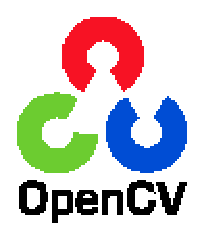
\includegraphics[scale=1]{img/opencv/logo.eps}
		\caption[OpenCV Logo]{OpenCV Logo}
		\label{opencv_logo}
		\end{center}
	\end{figure}

	The qualities described above as well as its optimization of various algorithms make this library an extremely useful asset for robotic vision projects. 
	In this project the C++ interface of the OpenCV library has been used. 
	The functionalities provided by this library are used in all the 2D data processing. 
	The next paragraph details the operations for which this library has been used. 

		\begin{itemize}
		\item\textbf{Segmentation of the 2D ROI (Region Of Interest)\\ }

		This library allows to crop the original raw image coming from the RGB-D sensor. 
		In our application, the segmentation is done around the user's hand. 
		For further details please read section \ref{roi_segmenter_2d}. 
		

		\item\textbf{ {Keypoints and descriptors extraction\\ }}

		 The OpenCV library implements multiple optimized state of the art algorithms. 
		 Among them, there are a number of descriptor extractors that has been already presented in chapter \ref{state_of_the_art}. 
		 The Oriented FAST and Rotated BRIEF (ORB)\cite{orb} algorithm is being used in this project due to its open-sourceness, and robustness / speed relation. 
		 More information about the different algorithms implemented in OpenCV used to extract the descriptors can be found in section \ref{feature_extraction}.


		\item\textbf{ {Descriptors matching\\ } }

		There are different matchers that might be used and that are implemented in the OpenCV library.
		The FlannBasedMatcher and the BruteForceMatcher are the two most used matchers due to its speed. 
		In this project, a FlannBasedMatcher (Fast Library for Approximate Nearest Neighbors Based Matcher) is being used for this purpose. 
		It is faster than the BruteForceMatcher specially for larger datasets. 
		It was selected to allow the use of more objects without losing efficiency. 
		\end{itemize}

	\subsection{Point Cloud Library (PCL)}
\label{pcl}
PCL is a standalone library that is open source and implements state-of-the-art algorithms related to 2D and 3D image and point cloud processing. \\
\begin{figure}[h]
	\begin{center}
    \includegraphics[scale=0.1]{img/pcl/pcl_logo.png}
	\caption[PCL Logo]{PCL Logo}
	\end{center}
\end{figure}

It is released under a BSD license, being free for commercial and research use. Is cross-platform and currently has been successfully compiled on Linux, MacOS, Windows, Android and iOS. \\

The library is divided in smaller code libraries that can be compiled separately. This modularity allows the PCL introduction on platforms with size constrains or that has a reduce computational size. \cite{Rusu_ICRA2011_PCL}
\\



\begin{figure}[h]
	\begin{center}
    \includegraphics[scale=0.4]{img/pcl/pcl_dependency.png}
	\caption[PCL graph of libraries]{PCL graph of code libraries and their relations}
	\end{center}
\end{figure}

		The Point Cloud Library is used within the software to perform transformations in the input point clouds and to perform descriptor extraction and matching in this data. 
		\\

		More specifically, PCL is used in the following processes: 

		\begin{itemize}
			\item{\textbf{Segmentation of the ROI (Region Of Interest)\\ }}

			This library allows to crop the original raw point cloud coming from the RGB-D sensor. In this application, the region cropped is the one around the hand being used. More information about this operation can be found in the \ref{roi_segmenter_3d} section. 
			

			\item{\textbf{ Keypoints and descriptors extraction\\ }}

			 The PCL library implements multiple optimized state of the art algorithms. Among them, there are a number of descriptor extractors such as PFH, FPFH or LINEMOD. In this project, the PFH descriptor is used due to its speed. More information about the different 3D descriptors implemented in PCL can be found in the section  \ref{feature_extraction}.


			\item {\textbf{Descriptors matching\\ }}

			There are different algorithms that allow to match the information provided by the descriptors, such as knn search or radius search. For further information about the type of matcher used in the present thesis, please visit the section \ref{learner_recognizer}
		\end{itemize}



	\subsection{Hardware}
		\label{technologies_hardware}

		The hardware needed in order to retrieve three-dimensional information is an RGB-D sensor compatible with the openni\_launch ROS package previously mentioned, and a computer running Linux. The information provided by this kind of device is more complete and makes the segmentation of the Region Of Interest easier. \\

		The sensor being used for the experiments presented in the following chapter is a Kinect of the Xbox 360. The reason of choosing this specific sensor is that it is cheaper than the other devices that include depth information. The main drawback with respect to other sensors such as the Asus Xtion PRO LIVE\cite{xtion} is that it needs a separate power plug to work, and also its size is bigger. 
		\\

		Further information about the Kinect's functioning may be found in section \ref{state_of_the_art}
		%  In this section the main components and functioning principles of the Kinect are going to be presented. Most of them are common with the other RGB-D sensors but others such as the VGA camera are optional, for example in some PrimeSense\cite{PrimeSense} models. 

		% \begin{figure}[h]
		% 	\begin{center}
		% 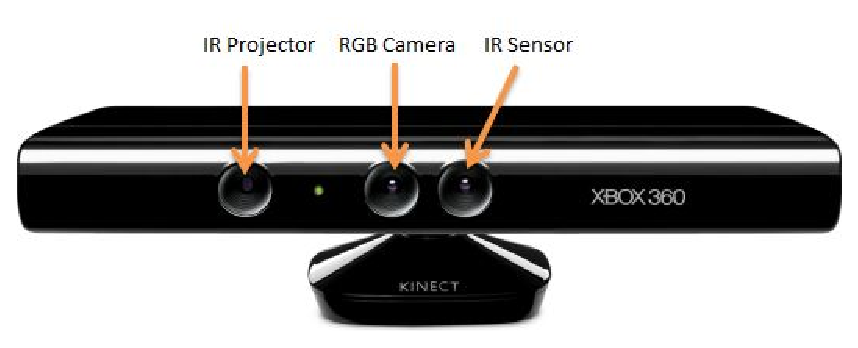
\includegraphics[scale=0.5]{img/kinect/kinect2.eps}
		% 	\caption[Kinect Sensors]{Kinect sensors: depth sensor and VGA camera location.}
		% 	\end{center}
		% \end{figure}


		% The parts that compose the Kinect sensor are the following: 

		% \begin{itemize}
		% 	\item{\textbf{VGA camera}}\\
		% 	The camera contained by the kinect has a pixel resolution of 640x480 and a frame rate of 30 fps. It is used mainly to provide the output data with the RGB components for each point. 
			
		% 	\item{\textbf{Depth sensor}\\
		% 	The depth sensor consists on an infra-red projector combined with a monochrome CMOS sensor. This latter measures the time it takes the light to come back after being reflected on the objects. Knowing the speed of light it can be easily obtained the distance of the objects from the depth sensor. 

		% 	\item{\textbf{Multi-array microphone}}\\
		% 	This array of four microphones are included because the kinect was designed as a gaming device. They are not used for the three-dimensional world retrieving. 

		% \end{itemize}

